\section{Application Protocols}\subsection{HTTP Server and Client SocketContext}

\begin{frame}{HTTP Server and Client \texttt{SocketContext}s}{Application Protocols}
  \begin{center}
    \begin{figure}
    \par\bigskip
    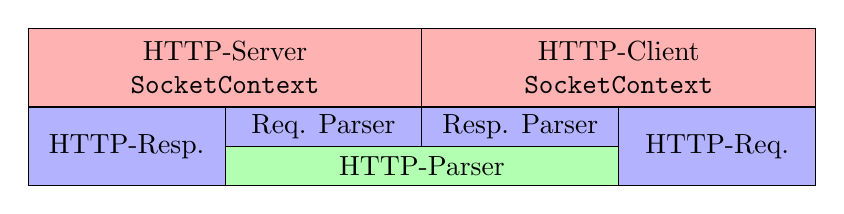
\begin{tikzpicture}
      \draw node [anchor=south, outer sep=0, inner sep=0, draw, fill=green!30, minimum width=5cm, minimum height=0.5cm] (http-p) {HTTP-Parser};

      \draw (http-p.south west) node[anchor=south east, outer sep=0, inner sep=0, draw, fill=blue!30, minimum width=2.5cm, minimum height=1cm] (http-res) {HTTP-Resp.};

      \draw (http-p.south east) node[anchor=south west, outer sep=0, inner sep=0, draw, fill=blue!30, minimum width=2.5cm, minimum height=1cm] (http-res) {HTTP-Req.};

      \draw (http-p.north west) node[anchor=south west, outer sep=0, inner sep=0, draw, fill=blue!30, minimum width=2.5cm, minimum height=0.5cm] (http-reqp) {Req. Parser};

      \draw (http-p.north east) node[anchor=south east, outer sep=0, inner sep=0, draw, fill=blue!30, minimum width=2.5cm, minimum height=0.5cm] (http-respp) {Resp. Parser};

      \draw (http-respp.north west) node[outer sep=0, inner sep=0, anchor=south west, fill=red!30, draw, minimum width=5cm, minimum height=1cm, align=center] (http-c) {HTTP-Client\\ \texttt{SocketContext}};

      \draw (http-reqp.north east) node[outer sep=0, inner sep=0, anchor=south east, fill=red!30, draw, minimum width=5cm, minimum height=1cm, align=center] (http-s) {HTTP-Server\\ \texttt{SocketContext}};
    \end{tikzpicture}
    \caption{HTTP server/client \texttt{SocketContext} in detail.}
  \end{figure}
  \end{center}\begin{itemize}
     \item HTTP \alert{request parser}
     \item HTTP \alert{response parser}
     \item \alert{Cookie} and \alert{query} support
     \item Connection management (0.9, 1.0, 1.1) (Connection: close, keep-alive, upgrade, ...)
     \item Real client side \alert{pipelining} support.
     \item Transfere-Encoding
      \begin{itemize}
        \item "`normal"' with Content-Length
        \item \alert{chunked} with \alert{trailer} support
      \end{itemize}
   \end{itemize}
\end{frame}
